\usection{Lecture 5: Pricing}
\newsection
\subsection*{Recap}
\begin{enumerate}
    \item Zero sum games
    \item Infinite population games - non-atomic traffic flow games.
\end{enumerate}
Recall in the last lecture we had in example \ref{pigon}:
\begin{center}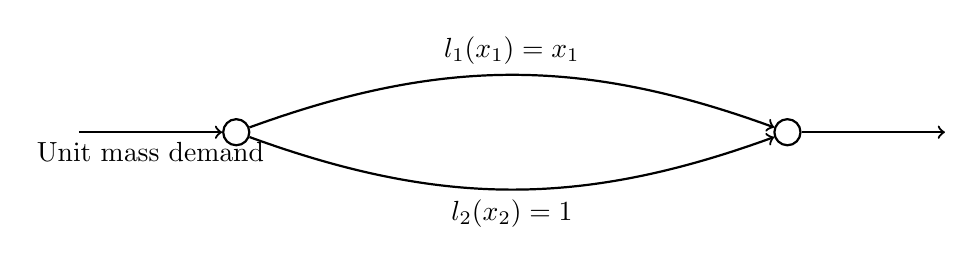
\begin{tikzpicture}
            
    \begin{scope}[every node/.style={circle,thick,draw}]
        \node (A) at (0,0) {};
        \node (B) at (7,0) {};
    \end{scope}
    \begin{scope}[every path/.style={->,thick}]
        \path [->] (-2,0) edge node[midway, below]{Unit mass demand}(A);
        \path [->] (A) edge [bend left=20] node[midway, above]{$l_1(x_1)=x_1$}(B);
        \path [->] (A) edge [bend right=20] node[midway, below]{$l_2(x_2)=1$}(B);
        \path [->] (B) edge (9,0);
    \end{scope}
    \end{tikzpicture}
\end{center}
Which had conflicting social optimal and equilibrium. However, we can introduce a price of $t_1=1/2$ to the upper route. i.e. $l_1(x_1)=x_1+1/2$ In this case, the equilibrium is when $x_1=x_2=1/2$. From an observer standpoint, we can disregard the tolls and get the social optimum strategy. However, for the drivers' standpoint, they still incur the full cost of $1$.

From an economic standpoint, we can disregard the cost of the toll. This is because the planner gets the toll fee of $(1/2)(1/2)=1/4$, but then this can be redistributed to everyone. 
\begin{remark}
    You can think of it `transfering' part of the cost of the bottom road to the top road to have $3/4$ cost each.
\end{remark}

We revisit the original model without tolls. Suppose that $x_1$ drivers are taking the top road and we consider the next driver ($x_1+\epsilon$?).

We define the social cost of the driver taking the top road as \[
\frac{d}{dx_1}x_1l_1(x_1)= x_1l_1'(x_1)+l_1(x_1).
\]
Previously each driver in the selfish equilibrium compares the costs $l_1(x_1)$ and $l_2(x_2)$. This is the second term in the cost. The first term is called \textbf{externality}.
\begin{atheorem}{Pigovian tax}{}
    Let $\tilde{l}_j(x)=xl_j'(x)+l_j(x)$. Under the new graph with costs $\tilde{l}_j$, the Wardrop eqiulibrium is the social optimal strategy with original costs.
\end{atheorem}
\corollary{
    The optimal toll cost for each road is $xl'(x)$. (up to a constant difference, but that is redistributed anyway.)
}

\subsection*{Finite number of users}
These leads to models that are known as congestion games. (Rosenthal, 1973)
\begin{remark}
    Rosenthal studied IEMS in Northwestern.
\end{remark}
\definition{Congestion Game}{
    A \textbf{congestion game} is a game with\begin{itemize}
        \item A set of players $R=\{1,2,\ldots,n\}$
        \item A set of resources $M=\{1,2,\ldots,m\}$
        \item For each $i\in R$, a set $S_i\subseteq 2^M$ denoting the subset of resources $i$ can use.
        \item Each resource has a cost of $c^j(x_j)$, where $x_j$ is the total number of players using the resource. The cost for player $i$ is $c_i(s_i,s_{-i})=\sum_{j\in s_i}c^j(x_j)$.
    \end{itemize}
}
\begin{aexample}{}{}
    
\begin{center}
    \begin{tikzpicture}
        
    \begin{scope}[every node/.style={circle,thick,draw}]
        \node [label=below:{player 1}](A) at (0,0) {};
        \node (B) at (7,0) {end};
        \node (C) at (3.5,2){};
        \node (D)[label=below:{player 2}] at (3.5,-2){};
    \end{scope}
    \begin{scope}[every path/.style={->,thick}]
        \path [->] (-2,0) edge (A);
        \path [->] (A) edge node[midway, above left] {$1$}(C);
        \path [->] (A) edge node[midway, below left] {$4$}(D);
        \path [->] (C) edge node[midway, above right] {$2$}(B);
        \path [->] (D) edge node[midway, below right] {$5$}(B);
        \path [->] (B) edge (9,0);
        \path [->] (D) edge node[midway, below right] {$3$}(C);
    \end{scope}
    \end{tikzpicture}\end{center}

Consider this game where both players want to reach the end.The roads are numbered 1 to 4. We have \begin{align*}
    M=&\{1,2,3,4,5\},\\
    S_1=&\{(1,2),(4,5),(4,3,2)\},\\
    S_2=&\{(3,2),5\}.
\end{align*}

\end{aexample}
\begin{aexample}{El Farol Bar Problem}{}
    10 people decide to go to the bar or go home. 
    If 6 or fewer go they have more fun than staying home. If 7 or more go, the bar is too crowded and they have less fun.
\end{aexample}
How do we model this as a congestion game?
We can model the resources as \[
\{\rm{bar}, \rm{home}\}.
\]
The strategy set of each player is \[
S_i=\{\rm{bar},\rm{home}\}
\]
Under this, the payoff is\[
\pi_i(s_i)=\begin{cases}
    1,&\textrm{if $x_{\rm{bar}}\leq 6$ and $s_i=$bar}\\-1,&\textrm{if $x_{\rm{bar}}\geq 7$ and $s_i=$bar}\\
    0,&\textrm{if $s_i=$home}\\
\end{cases}
\]
\begin{atheorem}{Rosenthal}{}
    Every congestion game has a pure strategy Nash equilibirum.
\end{atheorem}
We will \hyperref[]{prove this result} later.
\definition{Potential Game}{
    A game $G=(R,\{S_r\},\{\pi_r\})$ is a \textbf{potential game} if there is a function \[
    P:\prod_{r\in R} S_r\to \reals
    \]
    such that for all $r\in R$, $\bar{s}_{-r}$, and $x,z\in S_r$,
    \[
        \pi_r(x,\bar{s}_{-r})-\pi_r(z,\bar{s}_{-r})\geq 0 \iff P(x,\bar{s}_{-r})-P(z,\bar{s}_{-r})\geq 0
    \]
    with equality on the left iff equality on the right.
    In this case, we call $P$ a(an) \textbf{(ordinal) potential}.
    If \[
        \pi_r(x,\bar{s}_{-r})-\pi_r(z,\bar{s}_{-r})= P(x,\bar{s}_{-r})-P(z,\bar{s}_{-r}),
    \]
    we can $P$ an \textbf{exact potential}.
}
That is, a player benefits from changing strategies if and only if they can increase the potential.

Potential games exist.
\begin{aexample}{Cournot competition potential}{}
    $R$ firms choose $q_i\in[\epsilon,q_{\rm{max}}]$. The payoff for each company is \[
    \pi_i = q_i(P(Q)-c)
    \]
    where $Q=\sum q_r$.
    We let \[
        \Psi(q_1,\ldots, q_R) = \left(\prod_r q_r \right)(P(Q)-c).
    \]
    Then \begin{align*}
        \Psi(q_i,\bar{q}_{-i})-\Psi(\tilde{q}_i,\bar{q}_{-i})=&\left(\prod_{r\neq i}q_r\right)(q_i(P(Q_{-i}+q_i)-c)-\tilde{q}_i(P(Q_{-i}+\tilde{q}_i)-c))\\
        =&\left(\prod_{r\neq i}q_r\right)(\pi_i(q_i,\bar{q}_{-i})-\pi_i(\tilde{q}_i,\bar{q}_{-i})).
    \end{align*}
    This is \textit{almost} a potential game for $q_i\in[0,q_{\rm{max}}]$. Stricter conditions on $P$ can give potentials. 
\end{aexample} 

\begin{alemma}{}{}
    Every congestion game is a potential game
\end{alemma}

\begin{proof}[Sketch]
    We need to construct a potential for the congestion game. We claim \[
    P(\bar{s})= \sum_{j\in M}\sum_{1}^{x_j}C^j(k) 
    \]is a potential.
    Intuitively, take each resource $j$, then sum $C^j$ all the way from $1$ user to $x_j$ users.

    Suppose user $i$ using one $s_i$ and wants to switch towards using $\tilde{s}_i$. The change in cost is \[
        \pi_i(s_i,\bar{s}_{-i})-\pi_i(\tilde{s}_i,\bar{s}_{-i})=C^{s_i}(x_{s_i})-C^{\tilde{s}_i}(x_{s_i}).
    \]
    This is exactly the change in potential. (Apply an inductive argument).
\end{proof}
\begin{atheorem}{}{}
    Every potential game has a Nash equilibrium if the potential obtains its maximum for some strategy profile.
\end{atheorem}
\begin{proof}
    There is a maximal value for the potential function. Each player picks the strategy that maximize this potential function. This must be a Nash equilibirum.
\end{proof}
\corollary{
    Every finite potential game has at least one pure strategy Nash equilibrium. 
    Every game with a compact strategy set has at least one pure strategy Nash equilibrium.
}

\begin{proof}[Proof of Rosenthal]
    A congestion game has finite players and finite resources. Therefore it is a finite game. Since all congestion games are potential games, we are done.
\end{proof}


Nash equilibriums can be reached by using best response in potential games. I.e. choose one player and change his strategy to be the best response. The potential is strictly increasing, so has to be reached at some point. 